\section{Validating the Neural Posterior Estimator}
\label{sec:results}
In this section, we check whether our NPE is trained well and produces sensible and well-calibrated posteriors. We then describe how we use these posteriors to produce shear estimates in Sec.~\ref{sec:shear}.

\subsection{Training and Example Posteriors}
\label{ssec:training-examples}

Fig.~\ref{fig:npe-loss} shows the training and validation loss of our model over the course of training. Both losses decrease quickly in the first few epochs, then more slowly for the rest of training. The validation loss fluctuates in the first half of training, when the learning rate is still high, and settles down as the learning rate decreases. It is lowest at the final epoch, which we use for all of our analyses. Over the last 10 epochs, the validation loss only improves by 0.001, so the training has converged. It follows the training loss closely throughout, with no sign of overfitting.

\begin{figure}
    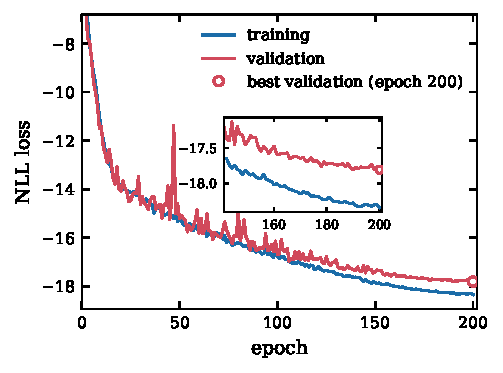
\includegraphics[width=\linewidth]{figs/training_loss.pdf}
    \caption{Training (blue) and validation (red) loss of our model as a function of epoch, i.e. the NLL of the true parameters in Eq.~(\ref{eqn:loss-unweighted}). The loss is computed in the rescaled parameter coordinates the flow is trained in, so only differences in the loss are meaningful. The validation loss is lowest at the final epoch (circle). Inset: a zoom-in on the last 60 epochs.}
    \label{fig:npe-loss}
\end{figure}

To see how our posteriors respond to the quality of the data, Fig.~\ref{fig:posterior-snr} shows the $g_1$--$g_2$ posterior of one galaxy from the Xu3 test set under different noise levels, keeping its parameters and noise realization fixed. Increasing the image SNR from $\rho_I=50$ to $\rho_I=200$ barely changes the posterior. In contrast, increasing the H$\alpha$ SNR from $\rho_S=8$ to $\rho_S=60$ shrinks $\sigma_{g_1}$ from 0.039 to 0.016. This is what we expect from KL. The image by itself only constrains the observed ellipticity, which is degenerate between the intrinsic shape and the shear, and at these image SNRs the observed ellipticity is likely already well measured. The spectra carry the kinematic information that breaks this degeneracy (Sec.~\ref{sec:kl-basics}), so it is expected that the precision of our measurements change most with spectral quality. This is consistent with \citep{KLInferenceI}, who also found that KL shape noise depends on the emission line SNR. The full 9D posterior of this galaxy is shown in Appendix~\ref{app:corner}.

\begin{figure*}
    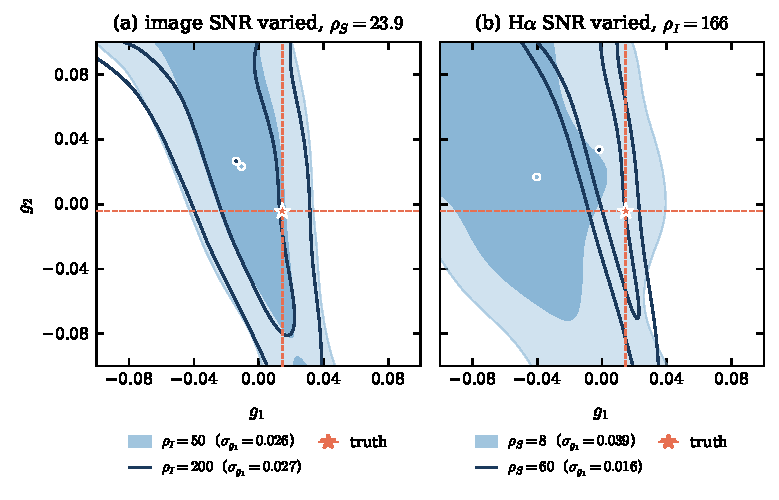
\includegraphics[width=\linewidth]{figs/posterior_snr.pdf}
    \caption{Shear posterior of one galaxy from the Xu3 test set (true $\cos i = 0.61$, true shear marked by the star and dashed lines) when the data quality is changed and everything else is kept fixed. (a) Image SNR $\rho_I = 50$ (filled) and $\rho_I = 200$ (lines), with the H$\alpha$ SNR at its catalog value $\rho_S = 23.9$. (b) H$\alpha$ SNR $\rho_S = 8$ (filled) and $\rho_S = 60$ (lines), with the image SNR at its catalog value $\rho_I = 166$. Contours enclose 68\% and 95\% of the posterior, estimated from $10^4$ posterior samples reweighted by the TF prior; dots mark the posterior means. \XW{Need to verify if the SNR choices are realistic. (perhaps a heat map instead)}}
    \label{fig:posterior-snr}
\end{figure*}

Once trained, our model draws $10^4$ posterior samples for a galaxy, including the TF reweighting, in about 0.3 seconds on a single NVIDIA V100 GPU. \XW{Can compare this with either published MCMC speeds or the current faster MCMC speeds, either way I'll need to ask for the number.}

\subsection{Posterior Calibration}
\label{ssec:calibration}

To test whether our NPE posteriors are well calibrated, we perform a coverage test. If the posteriors are correct, a credible interval at level $L$ should contain the true parameter value for a fraction $L$ of the test galaxies, e.g. 68\% of the 68\% credible intervals should contain the truth. Coverage tests are a standard way to validate approximate posteriors in simulation-based inference \citep{TrustCrisis}, and have been used to validate posteriors in weak lensing, including for NPE \citep{FieldLevelWL, NPEShear}.

We test the coverage of all credible levels at once with a P--P plot. For each test galaxy $i$ and shear component $g_k$, we compute the probability integral transform (PIT) $u_i$, the TF-weighted fraction of its $10^4$ posterior samples that lie below the true $g_k$. For correct posteriors, the true values are distributed like draws from the posteriors, so the PIT values are uniformly distributed between 0 and 1 \citep{CookGelmanRubin06, SBC}. The P--P plot shows the fraction of galaxies with $u_i \leq u$ as a function of $u$. In other words, it shows how often the true value falls below the $u$-quantile of its posterior, which should happen for a fraction $u$ of the galaxies, so the curve follows the diagonal for calibrated posteriors. If the posteriors are overconfident, the true values fall in their tails too often, which gives an S-shaped curve, while a bias in the posteriors shifts the curve to one side of the diagonal. Since the $\vcirc$ of our test galaxies are drawn from the same TFR as our TF prior (Sec.~\ref{ssec:test-set}), this test checks our NPE and the TF reweighting together.

With a finite number of test galaxies, the P--P curve scatters around the diagonal even for perfectly calibrated posteriors. To see how large this scatter can be, we use the Dvoretzky--Kiefer--Wolfowitz (DKW) inequality \citep{DKW56, Massart90}: for $N$ galaxies with exactly uniform PIT values, the P--P curve stays within $\pm\sqrt{\ln(2/0.05)/2N}$ of the diagonal for all $u$ with at least 95\% probability. In other words, this defines a band within which our curve should stay to be considered calibrated. For our $N=10^5$ Xu3 galaxies, this band is $\pm 0.0043$.

\begin{figure}
    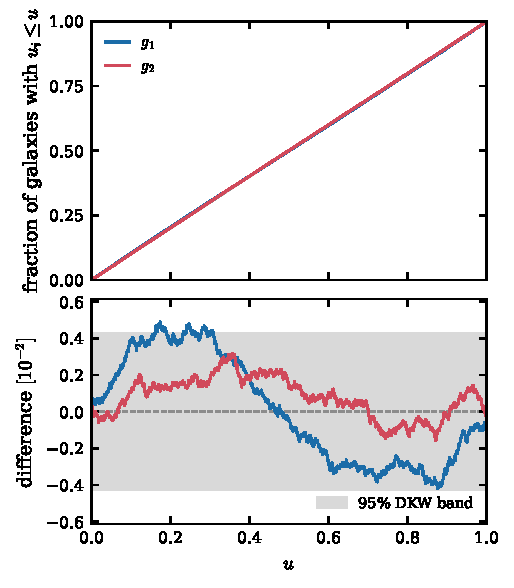
\includegraphics[width=\linewidth]{figs/pp_shear.pdf}
    \caption{P--P plot of the TF-weighted shear posteriors on the Xu3 test set ($10^5$ galaxies). Top: fraction of galaxies whose PIT value $u_i$, the fraction of posterior samples below the true shear, is at most $u$, for $g_1$ (blue) and $g_2$ (red). Calibrated posteriors follow the diagonal. Bottom: difference from the diagonal. The grey band is the 95\% DKW band, within which the curve of well calibrated posteriors stays with at least 95\% probability.}
    \label{fig:pp-shear}
\end{figure}

Fig.~\ref{fig:pp-shear} shows the P--P plot for $g_1$ and $g_2$. Both curves follow the diagonal closely and stay within the DKW band for nearly all $u$. Because the vast majority of the P--P curves stay within the DKW band, we consider our NPE shear posteriors to be well calibrated globally.

For the other seven parameters, we check the calibration at the 16th and 84th percentiles of each posterior, which correspond to $u = 0.16$ and $0.84$ in their P--P plots (Appendix~\ref{app:coverage}). All of them agree with the diagonal to within 1 percentage point, except for $\theta_\mathrm{int}$, whose true values fall in the tails of its posteriors somewhat too often. Since we marginalize over all parameters other than the shear when measuring shear, it is the calibration of $g_1$ and $g_2$ that matters in the end.

Note that this test checks the calibration averaged over the whole test set. It does not mean that the posterior of every galaxy, or of every subset of galaxies, is correct. We come back to this in Sec.~\ref{sec:discussion}, where we look at the calibration as a function of the true shear.
